This chapter contains the results of using the tool to evaluate the two
databases. First is a section showing the results for the evaluation of MariaDB,
following this is the results of PostgreSQL. Each of these sections contain the
results for all variations of the query as well as the different sample sizes used.

\subsection{MariaDB}
The evaluation of query variant 1 of the query for MariaDB can be seen in
Figure~\ref{fig:plot:mariadb:query1}.

\begin{figure}
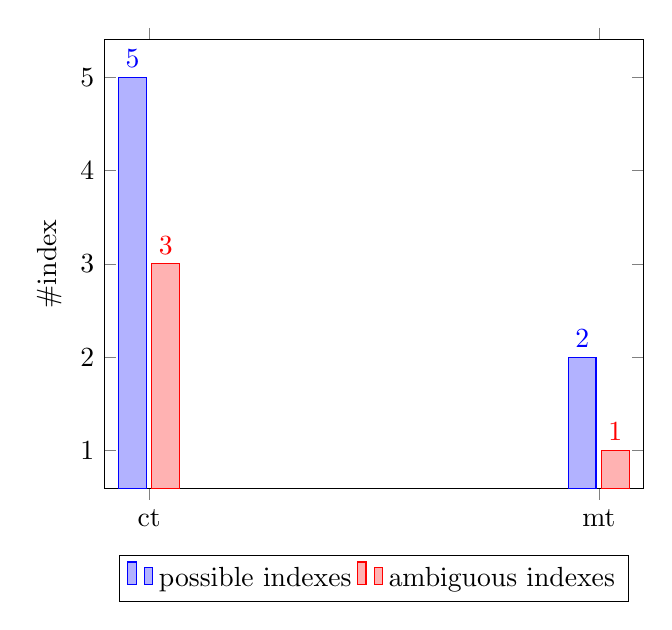
\begin{tikzpicture}
\begin{axis}[
    ybar,
    legend style={at={(0.5,-0.15)},
      anchor=north,legend columns=-1},
    symbolic x coords={ct,mt},
    ylabel={\#index},
    xtick=data,
    nodes near coords,
    nodes near coords align={vertical}
    ]
\addplot coordinates {(ct,5) (mt, 2)};
\addplot coordinates {(ct,3) (mt, 1)};
\legend{possible indexes, ambiguous indexes}
\end{axis}
\end{tikzpicture}
\caption[The index selections for MariaDB and query variant 1.]{The different
  indexes selected for MariaDB and the query variant 1, the possible index
  selections --- as in those considered by the query optimizer --- are shown next to
those actually selected.}\label{fig:plot:mariadb:query1}
\end{figure}

\subsection{PostgreSQL}
blahblah text